\documentclass[10pt,showpacs,preprintnumbers,footinbib,amsmath,amssymb,aps,prl,twocolumn,groupedaddress,superscriptaddress,showkeys]{revtex4-1}
\usepackage{graphicx}
\usepackage{dcolumn}
\usepackage{bm}
\usepackage[colorlinks=true,urlcolor=blue,citecolor=blue]{hyperref}
\usepackage{color}
\usepackage{listings}

\lstset{ %
  basicstyle=\footnotesize,        % the size of the fonts that are used for the code
  breakatwhitespace=false,         % sets if automatic breaks should only happen at whitespace
  breaklines=true,                 % sets automatic line breaking
  captionpos=t,                    % sets the caption-position to bottom
  deletekeywords={...},            % if you want to delete keywords from the given language
  escapeinside={\%*}{*)},          % if you want to add LaTeX within your code
  extendedchars=true,              % lets you use non-ASCII characters; for 8-bits encodings only, does not work with UTF-8
  frame=single,                    % adds a frame around the code
  keepspaces=true,                 % keeps spaces in text, useful for keeping indentation of code (possibly needs columns=flexible)
 % language=Python,                 % the language of the code
  morekeywords={*,...},           % if you want to add more keywords to the set
  numbers=left,                    % where to put the line-numbers; possible values are (none, left, right)
  numbersep=5pt,                   % how far the line-numbers are from the code
  showspaces=false,                % show spaces everywhere adding particular underscores; it overrides 'showstringspaces'
  showstringspaces=false,          % underline spaces within strings only
  showtabs=false,                  % show tabs within strings adding particular underscores
  stepnumber=1,                    % the step between two line-numbers. If it's 1, each line will be numbered
  tabsize=2,                       % sets default tabsize to 2 spaces
}


\begin{document}
\title{FYS3150 Computational Physics - Project 1}
\author{Nicholas Karlsen}

\begin{abstract}
  A look on two similar algorithms for solving an inhomogeneous second-order differential equation with a known analytical solution and comparing their efficiency to a standard LU-decomposition method. Found that the algorithms allow for greater precision and faster run-times.
\end{abstract}

\maketitle

\section{Introduction}
  When assuming spherical symmetry, the Poisson equation, eqn. \ref{poisson}

  \begin{equation}
    \label{poisson}
    \nabla^2 \mathbf \Phi = - 4\pi \rho (\mathbf r)
  \end{equation}
  can be reduced to the 1-dimensional second order inhomogeneous differential equation, eqn. \ref{diffeq1},
  by assuming spherical symmetry and scaling the problem.

  \begin{equation}
    \label{diffeq1}
    \frac{d^2u(x)}{dx^2} = f(x)
  \end{equation}

  A numerical solver for this equation not only allows us to solve the Poisson equation, but several other systems as well. In this report i have looked at one such solver, in both its general and specialized form and compared its speed to a solver which employs the LU-decomposition method in scipy and found that the solver was faster, but more importantly, allowed for a solution closer to what is allowed by the machine precision.


\section{Theory, algorithms and methods}
We have second order inhomogeneous differential equation, Eqn. \ref{differential_equation}
  \begin{equation}
    \label{differential_equation}
    \frac{d^2u(x)}{dx^2} = f(x)
  \end{equation}
  With boundary conditions $\ddot{u}(x) = f(x)$, $u(0) = u(1) = 0$ and $x \in (0, 1)$.

  If we let $f(x) = 100e^{-10x}$, then it can be shown analytically that the differential equation has a solution Eqn. \ref{diffeq anal sol}
  \begin{equation}
    \label{diffeq anal sol}
    u(x) = 1 - (1 - e^{-10})x - e^{-10x}
  \end{equation}

  This problem can also be solved numerically by discretization. By the use of taylor expansions, it can be shown that there is a discrete, iterative solution in the form Eqn. \ref{Discrete diffeq} \cite{lecture_notes}
  \begin{equation}
    \label{Discrete diffeq}
    - \frac{v_{i+1} + v_{i-1} + 2v_i}{h^2} = f_i
  \end{equation}
  where $h = 1/(n-1)$ is the step size for $n$ points and $V_i$ is the discretized form of $u(x)$.

  This problem can be written in the form 
  \begin{equation}
    A\vec v = \vec b
  \end{equation}
  Where $\textup A \in R^{n \times n}$ is a tridiagonal matrix with diagonal elements 2 and -1 (Eqn. \ref{A matrix}) and $\vec b =h^2(f_0, \dots, f_{n-1})$.
  \begin{equation}
    \label{A matrix}
    A = \left[ 
    \begin{matrix}
      2 & -1 & 0 & \dots  & \dots &0 \\
      -1 & 2 & -1 & 0 & \dots &  0 \\
      0 & -1 & 2 & -1 & \dots & \vdots  \\
      \vdots & \vdots & \vdots & \vdots & \vdots & -1\\
      \dots & \dots & \dots & \dots & -1 & 2
    \end{matrix}
    \right]
  \end{equation}

  By matrix multiplication, when we multiply   the $i$-th row of $A$ by $\vec v$, we get
  \begin{align}
  \begin{split}
 -1 v_{i -1} + 2v_i - 1v_{i+1}  &= -\left( v_{i+1} + v_{i-1} - 2v_i\right) 
                                \\&= h^2f_i
  \end{split}
  \end{align}

  Which is equivalent to the discretized differential equation Eqn. \ref{Discrete diffeq},
  showing that the differential equation can be solved as a linear algebra problem. 

  $A$ can be written more generally as
  \begin{equation}
    \label{A matrix general}
    A = \left[ 
    \begin{matrix}
      b_0 & c_0 & 0 & \dots  & \dots &0 \\
      a_1 & b_1 & c_1 & 0 & \dots &  0 \\
      0 & a_2 & b_2 & c_2 & \dots & \vdots  \\
      \vdots & \vdots & \vdots & \vdots & \vdots & c_{n-2}\\
      \dots & \dots & \dots & \dots & a_{n-1} & b_{n-1}
    \end{matrix}
    \right]
  \end{equation}
  By gauss elimination, we get the following set of equations for forward and backward substitutions respectively, which can be used to solve the system.

    \begin{align}
    \begin{split}
      \label{eqn:improved}
      \tilde b_i = b_i - \frac{1}{\tilde b_{i-1}}, 
      \enspace
      \tilde f_i = f_i + \frac{\tilde f_{i -1}}{\tilde b_{i-1}}, 
      \quad i &\in \{2, 3, \dots, n-2\} 
      \\
      v_{n-2} = \frac{\tilde f_{n-2}}{\tilde b_{n-2}}, &
      \\
      v_i = \frac{\tilde f_i + v_{i+1}}{\tilde b_i}, 
      \quad i &\in \{n-2, n-3, \dots, 1\}
    \end{split}
  \end{align}


  Or written in pseudocode/python;
  \lstinputlisting[language=Python, firstline=33, lastline=40]{code/gausselim.py}

  If we asume $\mathcal O(n)$ is such that $\pm$ numbers of order 0 become insignificant, then $\approx 9n$ FLOPS is required to compute this algorithm.

  For the special case, eqn. \ref{A matrix}, this algorithm can be further simplified by abusing the fact that the diagonal matrix elements $a_i, c_i$ are identical for all $i$. Resulting in the following sets of equations, \ref{eqn:improved}, for the substitutions.

  \begin{align}
    \begin{split}
      \label{eqn:improved}
      \tilde b_i = b_i - \frac{1}{\tilde b_{i-1}}, 
      \enspace
      \tilde f_i = f_i + \frac{\tilde f_{i -1}}{\tilde b_{i-1}}, 
      \quad i &\in \{2, 3, \dots, n-2\} 
      \\
      v_{n-2} = \frac{\tilde f_{n-2}}{\tilde b_{n-2}}, &
      \\
      v_i = \frac{\tilde f_i + v_{i+1}}{\tilde b_i}, 
      \quad i &\in \{n-2, n-3, \dots, 1\}
    \end{split}
  \end{align}
  This simplification results in $\approx 6n$ flops required to solve the problem, $67\%$ less flops than the general algorithm.



\section{Results and discussions}
  The implementation of the code discussed in the previous section can be found on my github: \url{https://github.com/nicholaskarlsen/FYS3150}. The code is in its entirety written in python, both due to how quick it is to implement and (mostly) because i am not yet comfortable enough with a more efficient language yet to use anything else. In order to offset some of the shortcomings of python i added some level of optimization using the JIT flag provided in the numba package.


  \begin{figure}[h!]
    \center
    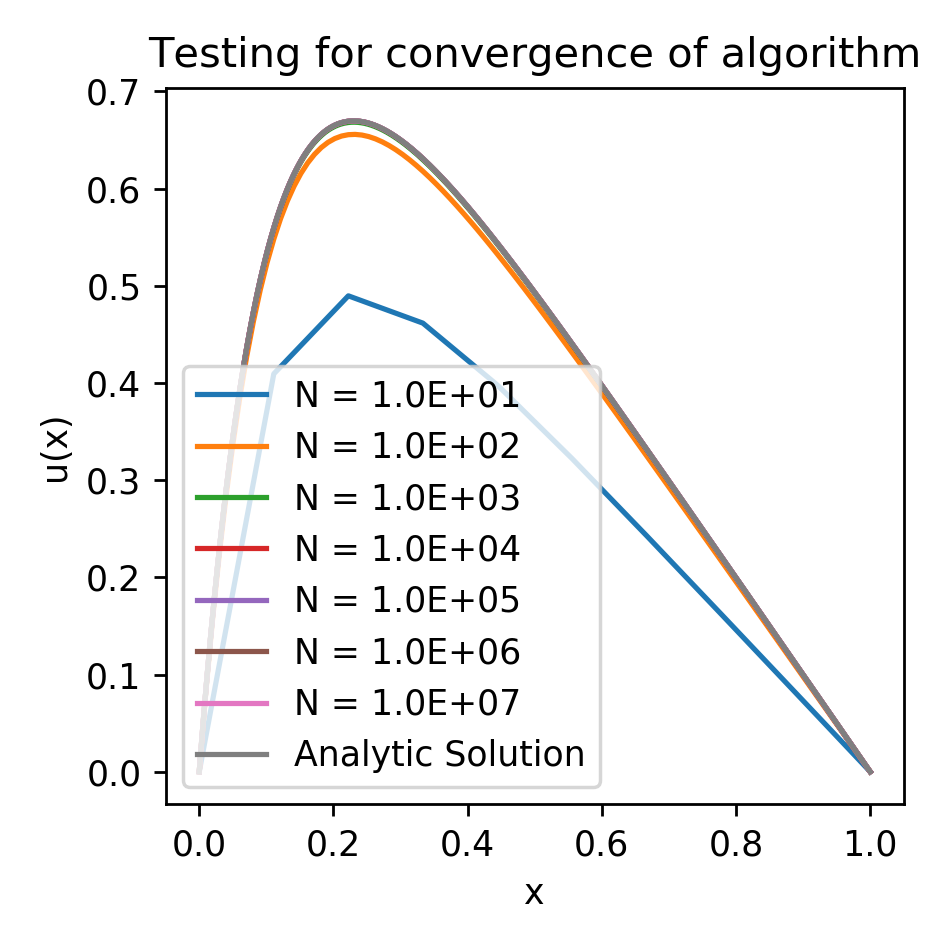
\includegraphics[scale=.7]{figs/ex1c_compare.png}
    \caption{A plot of the numeric solution for different N and the analytic solution.}
    \label{fig:compare}
  \end{figure}

  \begin{figure}[h!]
    \center
    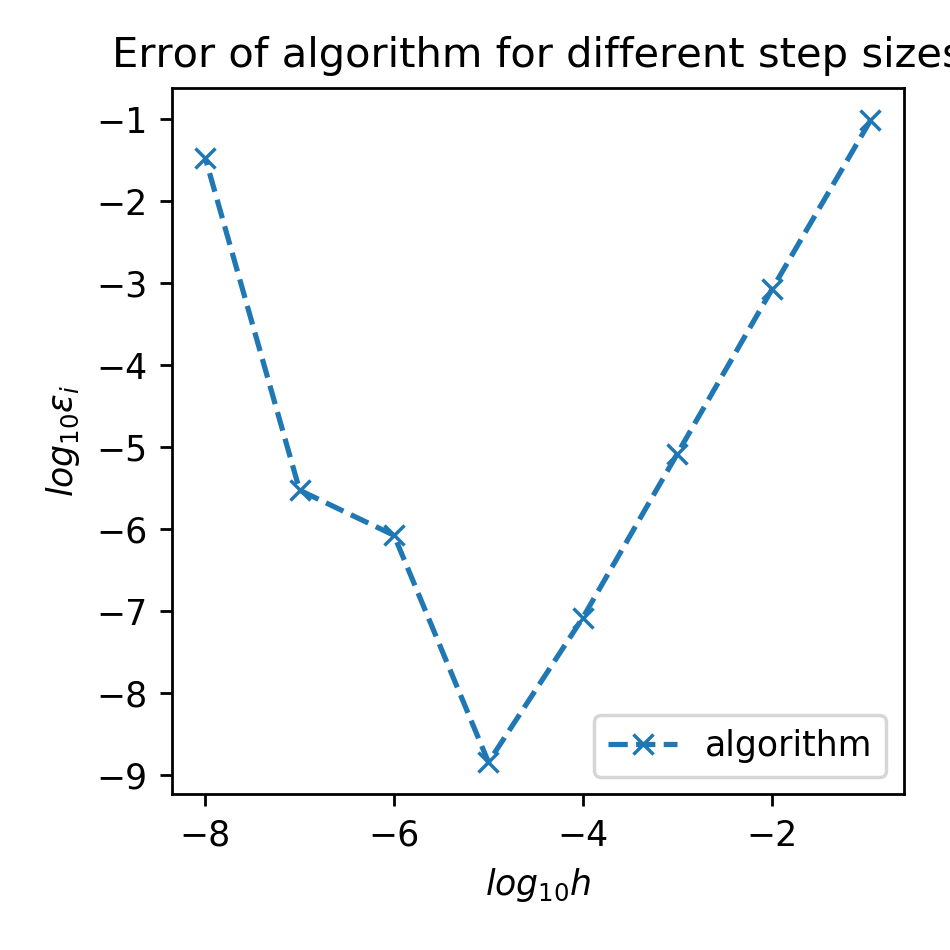
\includegraphics[scale=.7]{figs/ex1e_err.png}
    \caption{How the error evolves for smaller step sizes when comparing the general algorithm to the analytic solution}
    \label{fig:error}
  \end{figure}

  \begin{figure}[h!]
    \center
    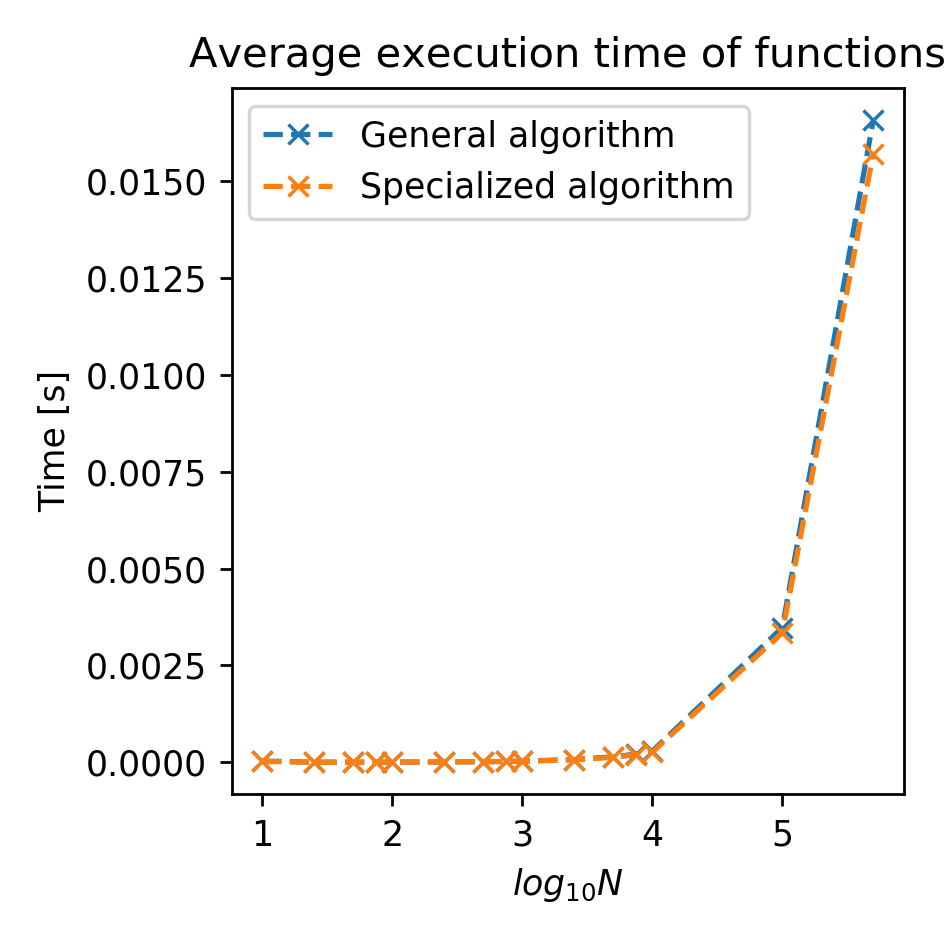
\includegraphics[scale=.7]{figs/ex1d_time.png}
    \caption{The average execution time of 10 function calls on my computer}
    \label{fig:time}
  \end{figure}

  \begin{figure}[h!]
    \center
    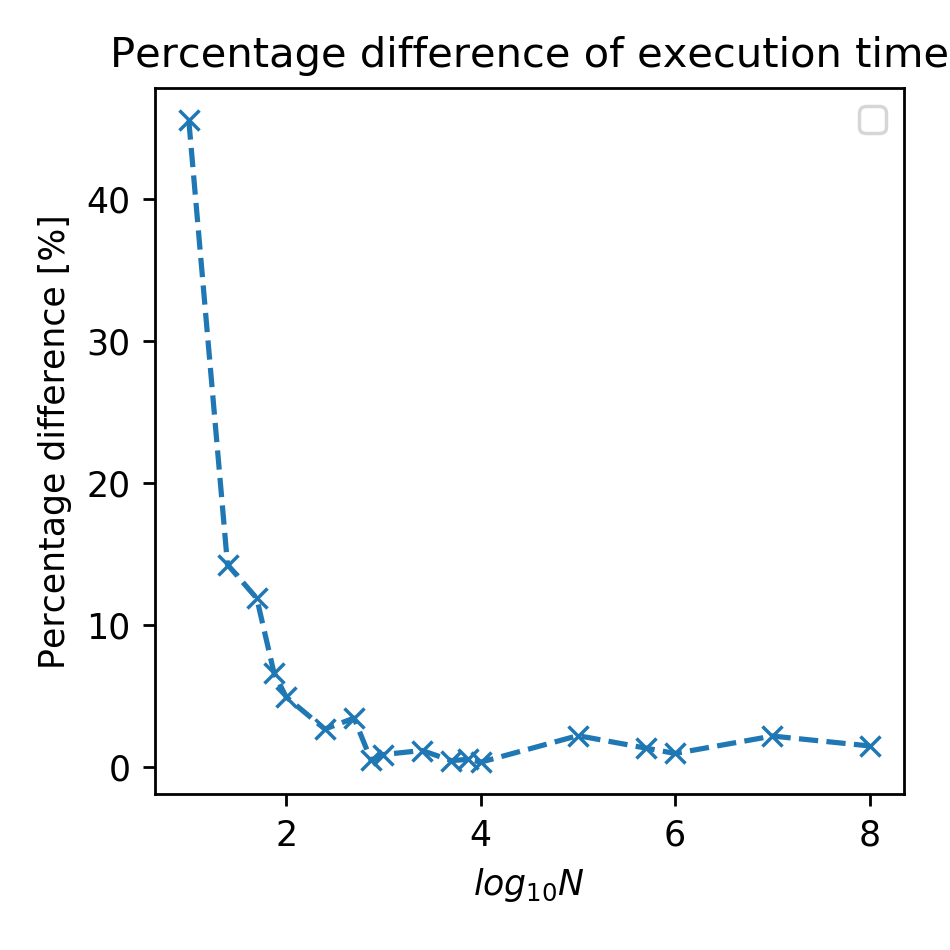
\includegraphics[scale=.7]{figs/ex1d_timediff.png}
    \caption{Percentage difference between the execution times of the general and specialized algorithms on my computer}
    \label{fig:timediff}
  \end{figure}

  As seen in Figures \ref{fig:compare}, \ref{fig:error}, the algorithm converges towards the analytic solution with a relative error, $\epsilon$ such that $\log_{10}\epsilon \propto \log_{10} h$ for $\log_{10}h \gtrapprox 5$ which is where loss of precision due to the finite representation of numbers in computers becomes relevant. As such, it is ideal to chose $h\approx 10^{-5}$ when precision is the main priority, but never $h\lessapprox10^{-5}$ as the extra computation time is simply wasted.

  In Figures \ref{fig:time}, \ref{fig:timediff} we see how the execution time of the different algorithms compare for different $N$. This data does not reflect the expected $66\%$ performance increase predicted based on the number of FLOPS. Therefore I suspect there may be something wrong with either the way I'm timing the functions, or the numpy calls prior to the backward/forward loops may be the dominating factor in the execution time. Due to the way i wrote gausselim.general(), i was somewhat limited in the way i could time my function without causing errors, and i did not have the time to explore different options / restructure my code.

  Comparing them to the execution time for the scipy LU-decomposition solver however shows that the custom custom algorithms perform very well. First and foremost, the LU-decomposition method is much more limited by memory. On my computer, with 16GiB of memory, the largest exponent of 10 sized matrix that could be solved without running out of memory was $10^4$. The execution time also rises grows quicker than for the custom algorithms.

\section{Conclusions}

  In conclusion, it has become apparent that there is a lot of time and memory to be saved by remodeling a problem to a more efficient form rather than blindly using a standard solver, thus enabling us to solve problems that may have otherwise not been feasible given our resources. Further, one must be critical when lowering the step sizes of numerical solvers such that machine precision does not become a dominant term in its error.


\begin{thebibliography}{99}
\bibitem{lecture_notes} M.~Hjorth-Jensen, Computational Physics - Lecture Notes 2015, (2015).
\end{thebibliography}


\end{document}